\documentclass[11pt]{article}
\usepackage[margin=1in]{geometry}
\usepackage{amsmath,amssymb}
\usepackage{graphicx}
\usepackage{booktabs}
\usepackage[hidelinks]{hyperref}
\usepackage{caption}
\captionsetup{font=small}
\graphicspath{{figures/}}

\title{\vspace{-2.5em}Belief-State Geometry in Transformers:\\
Reproduction and Unsupervised Recovery via Observable Operator Models}
\author{}
\date{}

\begin{document}
\maketitle
\vspace{-3em}

\section{Introduction}

Shai et al.\cite{shai2024} show that a transformer trained on sequences from a hidden
data-generating process linearly represents, in its residual stream, the geometry of \emph{belief states}: 
the Bayesian posterior distributions over the generator's hidden states. The geometry is characterised by 
the \emph{mixed-state presentation} (MSP): each history $w$ induces a belief $b(w)$ over the hidden states, 
and the set of reachable beliefs forms a characteristic structure in the probability simplex over the 
hidden states (for classical data-generating processes)\cite{riechers2025}.
\\\\
This work reproduces the supervised results and contributes an \emph{unsupervised} estimator
that recovers the belief-state geometry from activations and the network's own next-token
probabilities alone, without ground-truth belief labels or knowledge of the generating
process, using observable operator models (OOMs).
We present supervised and unsupervised belief state recovery on two processes; \emph{Mess3}, a
$3$-state dense process with Sierpinski fractal geometry, and \emph{RRXOR}, a $5$-state
synchronising process with $36$ discrete belief states.
\\\\
Both processes are trained using the paper's architecture ($d_{\mathrm{model}}{=}64$, $4$ layers,
$1$ head, $d_{\mathrm{mlp}}{=}256$, ReLU, LayerNorm, SGD) for $10^6$ steps.
Throughout, we use prefix deduplication: since causal attention ensures identical contexts
produce identical activations, each unique prefix appears once (weighted by its total frequency)
rather than at every position. We weight all regressions by prefix probability $P(w)$, following~\cite{riechers2025}, 
to give priority to the model's learned geometry in high-probability regions.
\\\\
A limitation of the supervised approach is requiring knowledge of the data-generating process, which prevents us 
from applying this approach to large language models. If we could recover the belief geometry in an unsupervised 
way this would address this limitation. If transformers truly represent belief-state geometry linearly in their 
residual streams, then this geometry should be recoverable without labels or access to the generating process. 
Success on these controlled experiments would suggest that the approach could extend to large language
models.
\section{Results: Supervised vs.\ Unsupervised Recovery}

\subsection{The unsupervised estimator}
\label{sec:estimator}

The estimator recovers the belief subspace from activations and the network's own
softmax, using the \emph{observability matrix} of an observable operator model (OOM) \cite{jaeger2000},
but estimated in activation space. We refer to this estimator as the spectral-OOM.
This differs from Baum-Welch (EM) \cite{baum1970}, which fits a generative HMM to the token
sequence rather than reading the representation out of the network.

\paragraph{Linearising the belief update.}
The network encodes belief affinely, $a(w) = b(w)\Psi + c$, where $\Psi$
is the linear embedding and $c$ is a constant offset. Because every regression 
below is fit with an intercept (equivalently, on $P(w)$-centered activations), 
the offset $c$ is absorbed and the operators are estimated on the linear part $b(w)\Psi$.
The Bayesian update is projective (Eq.~\eqref{eq:update}),
\begin{equation}
b(wx)=\frac{b(w)T^x}{b(w)T^x\mathbf{1}}, \qquad P(x|w)=b(w)T^x\mathbf{1}.
\label{eq:update}
\end{equation}
a homography: a linear map $b(w)\mapsto b(w)T^x$ followed by a normalisation that divides
by a linear functional of $b(w)$. The ratio is non-linear in $b(w)$, and hence in
$a(w)$, so no fixed matrix relates consecutive activations across all prefixes $w$.
\\\\
However, observe that the \emph{normalising denominator is exactly the next-token
probability} $P(x|w)=b(w)T^x\mathbf{1}$, which is the network's softmax output.
Multiplying both sides by $P(x|w)$ removes the non-linearity, giving us
\begin{equation}
b(wx)\,P(x|w)=b(w)\,T^x,
\label{eq:cleared}
\end{equation}
whose right-hand side is now linear in $b(w)$. Right-multiplying~\eqref{eq:cleared} by
$\Psi$ rewrites it in activation coordinates. On the left, $P(x|w)$ is a scalar and
$b(wx)\Psi=a(wx)$, giving $P(x|w)\,a(wx)$. On the right, inserting $\Psi\Psi^{+}$
(the identity on the belief row-space when $\Psi$ has full row rank $d$, i.e.\ the
encoding is injective) regroups $b(w)\Psi$ into $a(w)$:
\[
b(w)\,T^x\,\Psi
=b(w)\,\big(\Psi\Psi^{+}\big)\,T^x\,\Psi
=\big(b(w)\Psi\big)\big(\Psi^{+}T^x\Psi\big)
=a(w)\,A_x,
\qquad A_x:=\Psi^{+}T^x\Psi .
\]
Equating the two sides yields a single fixed operator $A_x$ relating every parent
activation $a(w)$ to its rescaled child $P(x|w)\,a(wx)$ (where child activation means the appended-token
activation $a(wx)$)
\begin{equation}
a(w)\,A_x \;\approx\; P(x|w)\,a(wx).
\label{eq:linearise}
\end{equation}
The relation is approximate because $\Psi$ is unknown, belief is only approximately encoded,
and $A_x$ are estimated from finite data. The map $A_x=\Psi^{+}T^x\Psi$ is simply the hidden-state 
operator $T^x$ expressed in activation coordinates. Crucially, the rescaling by the network's own 
$P(x|w)$ is what absorbs the prefix-dependent normaliser that made the update projective, leaving 
a relation that is \emph{linear} in the sense that one matrix $A_x$ holds for all $w$. Each $A_x$ 
is thus estimable by a single ($P(w)$-weighted) linear regression over transition pairs 
$\big(a(w),\,a(wx)\big)$ rescaled by $P(x|w)$, no supervised targets are required.

\paragraph{Recovering the subspace.}
The operators $A_x$ of Eq.~\eqref{eq:linearise} advance the state \emph{within}
activation space; we also need a \emph{readout} from a state to what it predicts. Let $C$ 
be the ($P(w)$-weighted) ridge regression of activations $a(w)$ onto the softmax row $P(\cdot\,|\,w)$, 
the one-step observable. It is linear in belief because $P(x|w)=b(w)T^x\mathbf{1}$ (Eq.~\eqref{eq:update}) 
is a linear functional of $b(w)$, so the full softmax row is a linear image of $b(w)$ and hence of $a(w)$. 
We fit $C$ as a linear map rather than reuse the network's own activation-to-softmax map because 
the latter is non-linear (the softmax) and so cannot be composed into the matrix products below. 
$C$ is the best linear readout to the next-token probability simplex, and the SVD acts on matrices. 
Both $C$ and $\{A_x\}$ are fit by the same regression from one pass over the prefix tree, 
independently and in either order. Their only targets are the network's softmax and (rescaled) child
activations.
\\\\
The pair $(C,\{A_x\})$ is the activation-space analogue of the output map and dynamics of
a linear system. $C$ says what is seen now, $A_x$ says how the state evolves, so $A_x C$
is what is seen one step ahead, $A_x A_y C$ two steps ahead, and so on. Composing the
$A_x$ preserves linearity in $b(w)$, so every such multi-step observable is again linear
in belief. Stacking them up to a horizon $L$ gives the \emph{observability matrix}
\begin{equation}
\mathcal{O}=\big[\,C \;\big|\; (A_x C)_{x} \;\big|\; (A_x A_y C)_{x,y}
\;\big|\;\cdots\;\big|\;(A_{x_1}\!\cdots A_{x_L} C)_{x_1,\dots,x_L}\,\big],
\label{eq:obsmat}
\end{equation}
indexed over all words up to length $L$. This is the (word-indexed)
control-theoretic observability matrix of the estimated OOM; $L$ is taken large enough
that $\mathcal{O}$ reaches its full rank, i.e.\ enough future to make the hidden states
distinguishable.
\\\\
The column space of $\mathcal{O}$ is the image of belief space under the encoding, so it
spans exactly the belief-carrying directions of activation space, the \emph{belief subspace},
isolating it from the rest of the residual stream. Its dimension, the numerical rank of 
$\mathcal{O}$, is the model order. For an observable (minimal) process this equals the number 
of hidden states, while a weakly observable process exposes only its observable part and can rank 
below the true state count (see Section~\ref{sec:rrxor}, RRXOR). An SVD $\mathcal{O}=U\Sigma V^\top$ 
then does two things: the singular-value spectrum locates the effective rank $d$ (the elbow giving 
the model order), and the leading left singular vectors $B=U_{:,1:d}$ furnish an orthonormal basis for the
belief subspace, which we use to project activations. 
Recovering a state subspace via the SVD of a matrix of observable statistics is the standard spectral-learning 
route \cite{hsu2012, thon2015}. There they factor the past$\times$future Hankel matrix, whereas 
here we build its observability factor directly from learned operators in activation space. 
The procedure uses only activations, softmax, and the prefix tree.

\paragraph{Recovering the subspace from the past: the controllability factor.}
The observability matrix~\eqref{eq:obsmat} stacks \emph{futures}: from a state, what is
predicted ahead. The dual object stacks \emph{pasts}: which states are \emph{reachable} by
driving the process forward from its start. Recall the forward (un-normalised) update of
Eq.~\eqref{eq:cleared}, $b(wx)\,P(x|w)=b(w)\,T^x$. Iterating from the stationary root belief
$b_0$ along a word $w=x_1\cdots x_k$ telescopes the scalars into the joint probability,
\begin{equation}
b(w)\,P(w)=b_0\,T^{x_1}T^{x_2}\cdots T^{x_k},
\qquad P(w)=\textstyle\prod_{i} P(x_i\mid x_1\cdots x_{i-1}),
\label{eq:reach}
\end{equation}
since each step contributes one conditional factor and the denominators telescope. The
right-hand side is linear in $b_0$: the un-normalised reachable state after word $w$ is just
$b_0$ pushed through the product operator $T^{w}:=T^{x_1}\!\cdots T^{x_k}$.

\paragraph{In activation coordinates.}
Right-multiply~\eqref{eq:reach} by $\Psi$ and insert $\Psi^{+}\Psi$ between every adjacent
pair of operators (the identity on the belief row-space when $\Psi$ has full row rank $d$):
\[
b_0\,T^{x_1}\!\cdots T^{x_k}\,\Psi
= \big(b_0\Psi\big)\big(\Psi^{+}T^{x_1}\Psi\big)\cdots\big(\Psi^{+}T^{x_k}\Psi\big)
= a_0\,A_{x_1}\!\cdots A_{x_k},
\]
with $a_0:=b_0\Psi$ the root activation and $A_x=\Psi^{+}T^{x}\Psi$ \emph{the same operators}
already estimated in Eq.~\eqref{eq:linearise}. Because the left side equals $a(w)\,P(w)$, this
gives the reachability relation
\begin{equation}
a_0\,A_{x_1}\!\cdots A_{x_k} \;\approx\; P(w)\,a(w),
\label{eq:reach-act}
\end{equation}
the exact dual of~\eqref{eq:linearise}: the observability blocks compose operators \emph{on the
right of} $C$ (futures read out forward), whereas reachability composes the \emph{same} operators
\emph{on the left of} $a_0$ (pasts driven forward from the root). No new operator fits are needed,
the controllability factor reuses $\{A_x\}$ and the single root activation $a_0$.

\paragraph{The controllability matrix.}
Stacking the reachable activations over all words up to horizon $L$ gives
\begin{equation}
\mathcal{R}=
\begin{bmatrix}
a_0\\[2pt]
(a_0 A_x)_{x}\\[2pt]
(a_0 A_x A_y)_{x,y}\\[2pt]
\vdots\\[2pt]
(a_0 A_{x_1}\!\cdots A_{x_L})_{x_1,\dots,x_L}
\end{bmatrix},
\label{eq:reachmat}
\end{equation}
each row the (un-normalised) activation reached by its word. Its \emph{row} space is the span of
reachable states in activation space, the reachable belief subspace; for a process whose start
state explores all of belief space this coincides with the column space of $\mathcal{O}$, both
equal the $d$-dimensional belief subspace, which is the activation-space statement of the
factorisation $H=\mathcal{R}\,\mathcal{O}^{\!\top}$ at rank $d$.

\paragraph{Estimation.}
Unlike the observability factor, $\mathcal{R}$ requires no per-word regression: each row is a
\emph{deterministic} product of the already-fitted $\{A_x\}$ applied to $a_0$. The only estimated
inputs are $a_0$ (the $P(w)$-weighted mean root activation, or the empirical activation at the
start token) and the operators themselves. In practice the rows should be \emph{$P(w)$-weighted}
exactly as the observability construction is, because~\eqref{eq:reach-act} produces the
\emph{un-normalised} $P(w)\,a(w)$, so high-probability prefixes already carry larger norm and
dominate the SVD, matching the weighting of $\mathcal{O}$ and of the supervised decode.

\subsection{Mess3}

\begin{figure}[!ht]
\centering
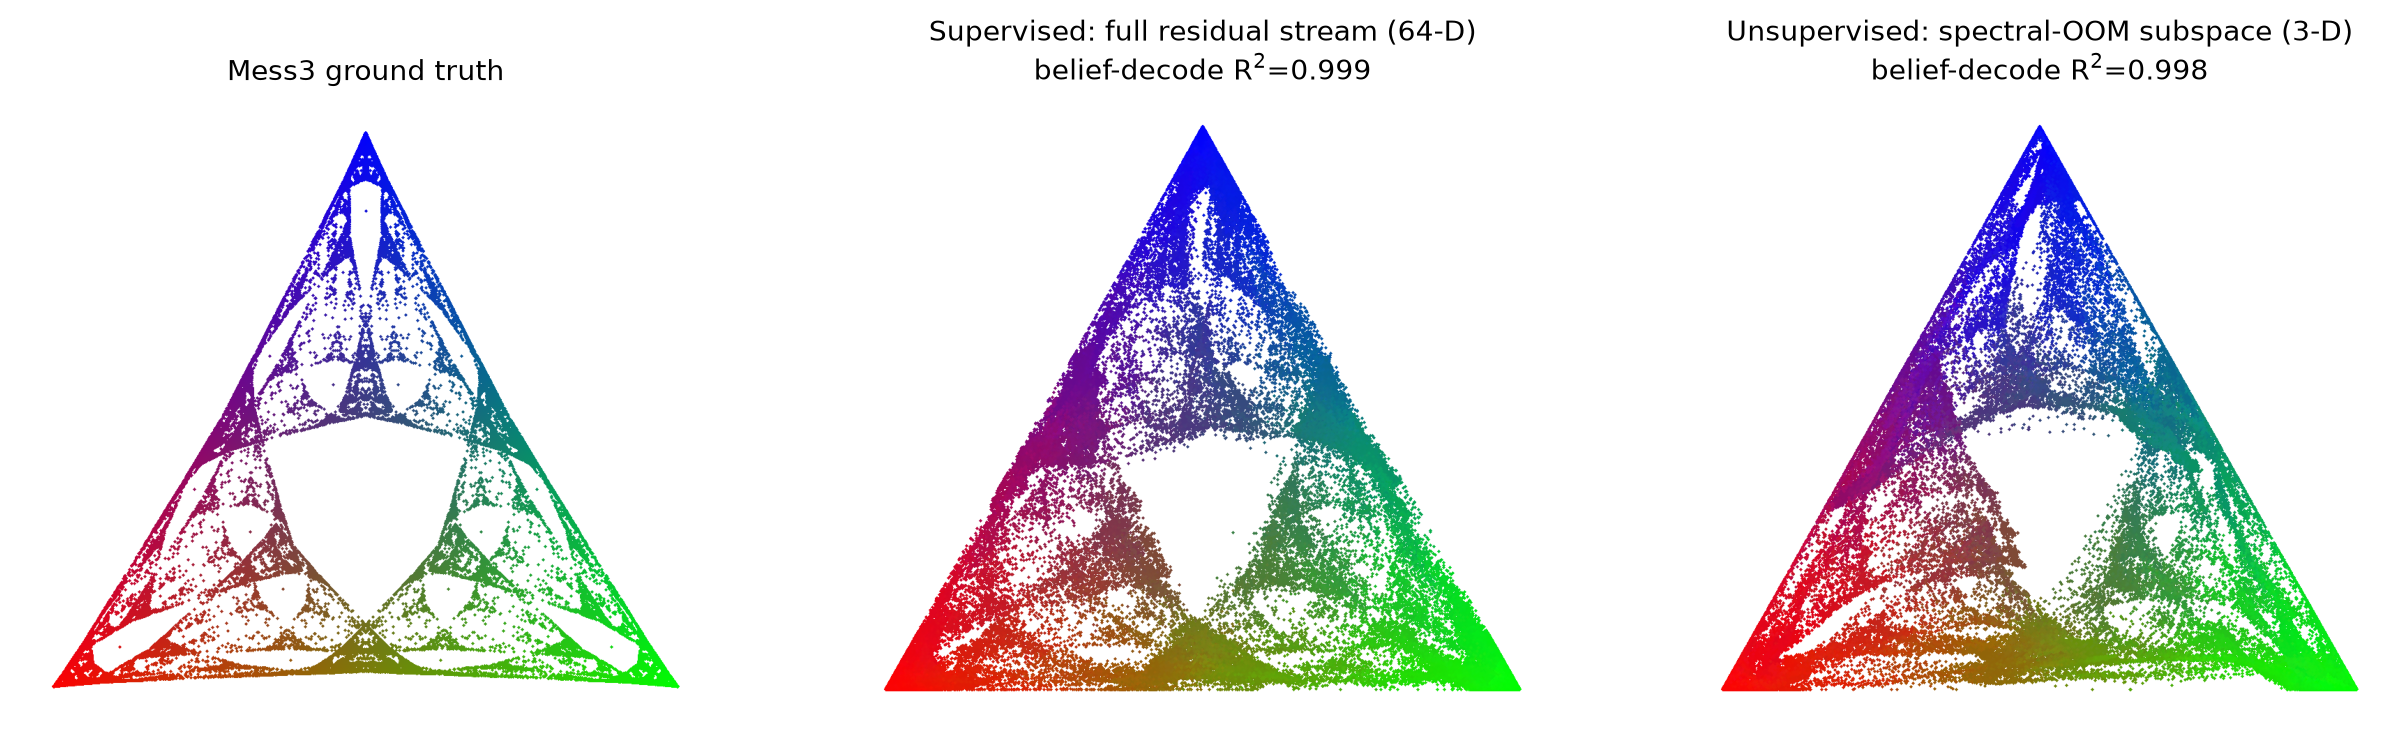
\includegraphics[width=0.9\textwidth]{fig1_mess3_principled.png}
\caption{\textbf{Mess3: ground truth, supervised, and unsupervised.}
Left: ground-truth belief geometry.
Centre: supervised decode from full $64$-D residual stream ($R^2=0.999$).
Right: unsupervised spectral-OOM subspace ($R^2=0.998$).
The estimator recovers the fractal nearly identically.}
\label{fig:mess3comp}
\end{figure}
\noindent For the Mess3 process, unsupervised recovery is nearly perfect.
The observability spectrum drops cleanly at $d=3$, and the recovered $3$-D subspace decodes
belief at $R^2=0.998$, almost as good as supervised.
The geometry emerges similarly during training (Figure~\ref{fig:mess3prog}) and survives
identical controls: both cross-validate on held-out prefixes and collapse under belief-label
(supervised) or softmax (unsupervised) shuffle (Figure~\ref{fig:mess3ctrl}).
The $30/70$ split is a slight change from the $20/80$ split in the original because the original
split provides too little data for unsupervised learning; its training unit is a transition 
(parent + all children), while supervised trains on single prefixes.

\begin{figure}[!ht]
\centering
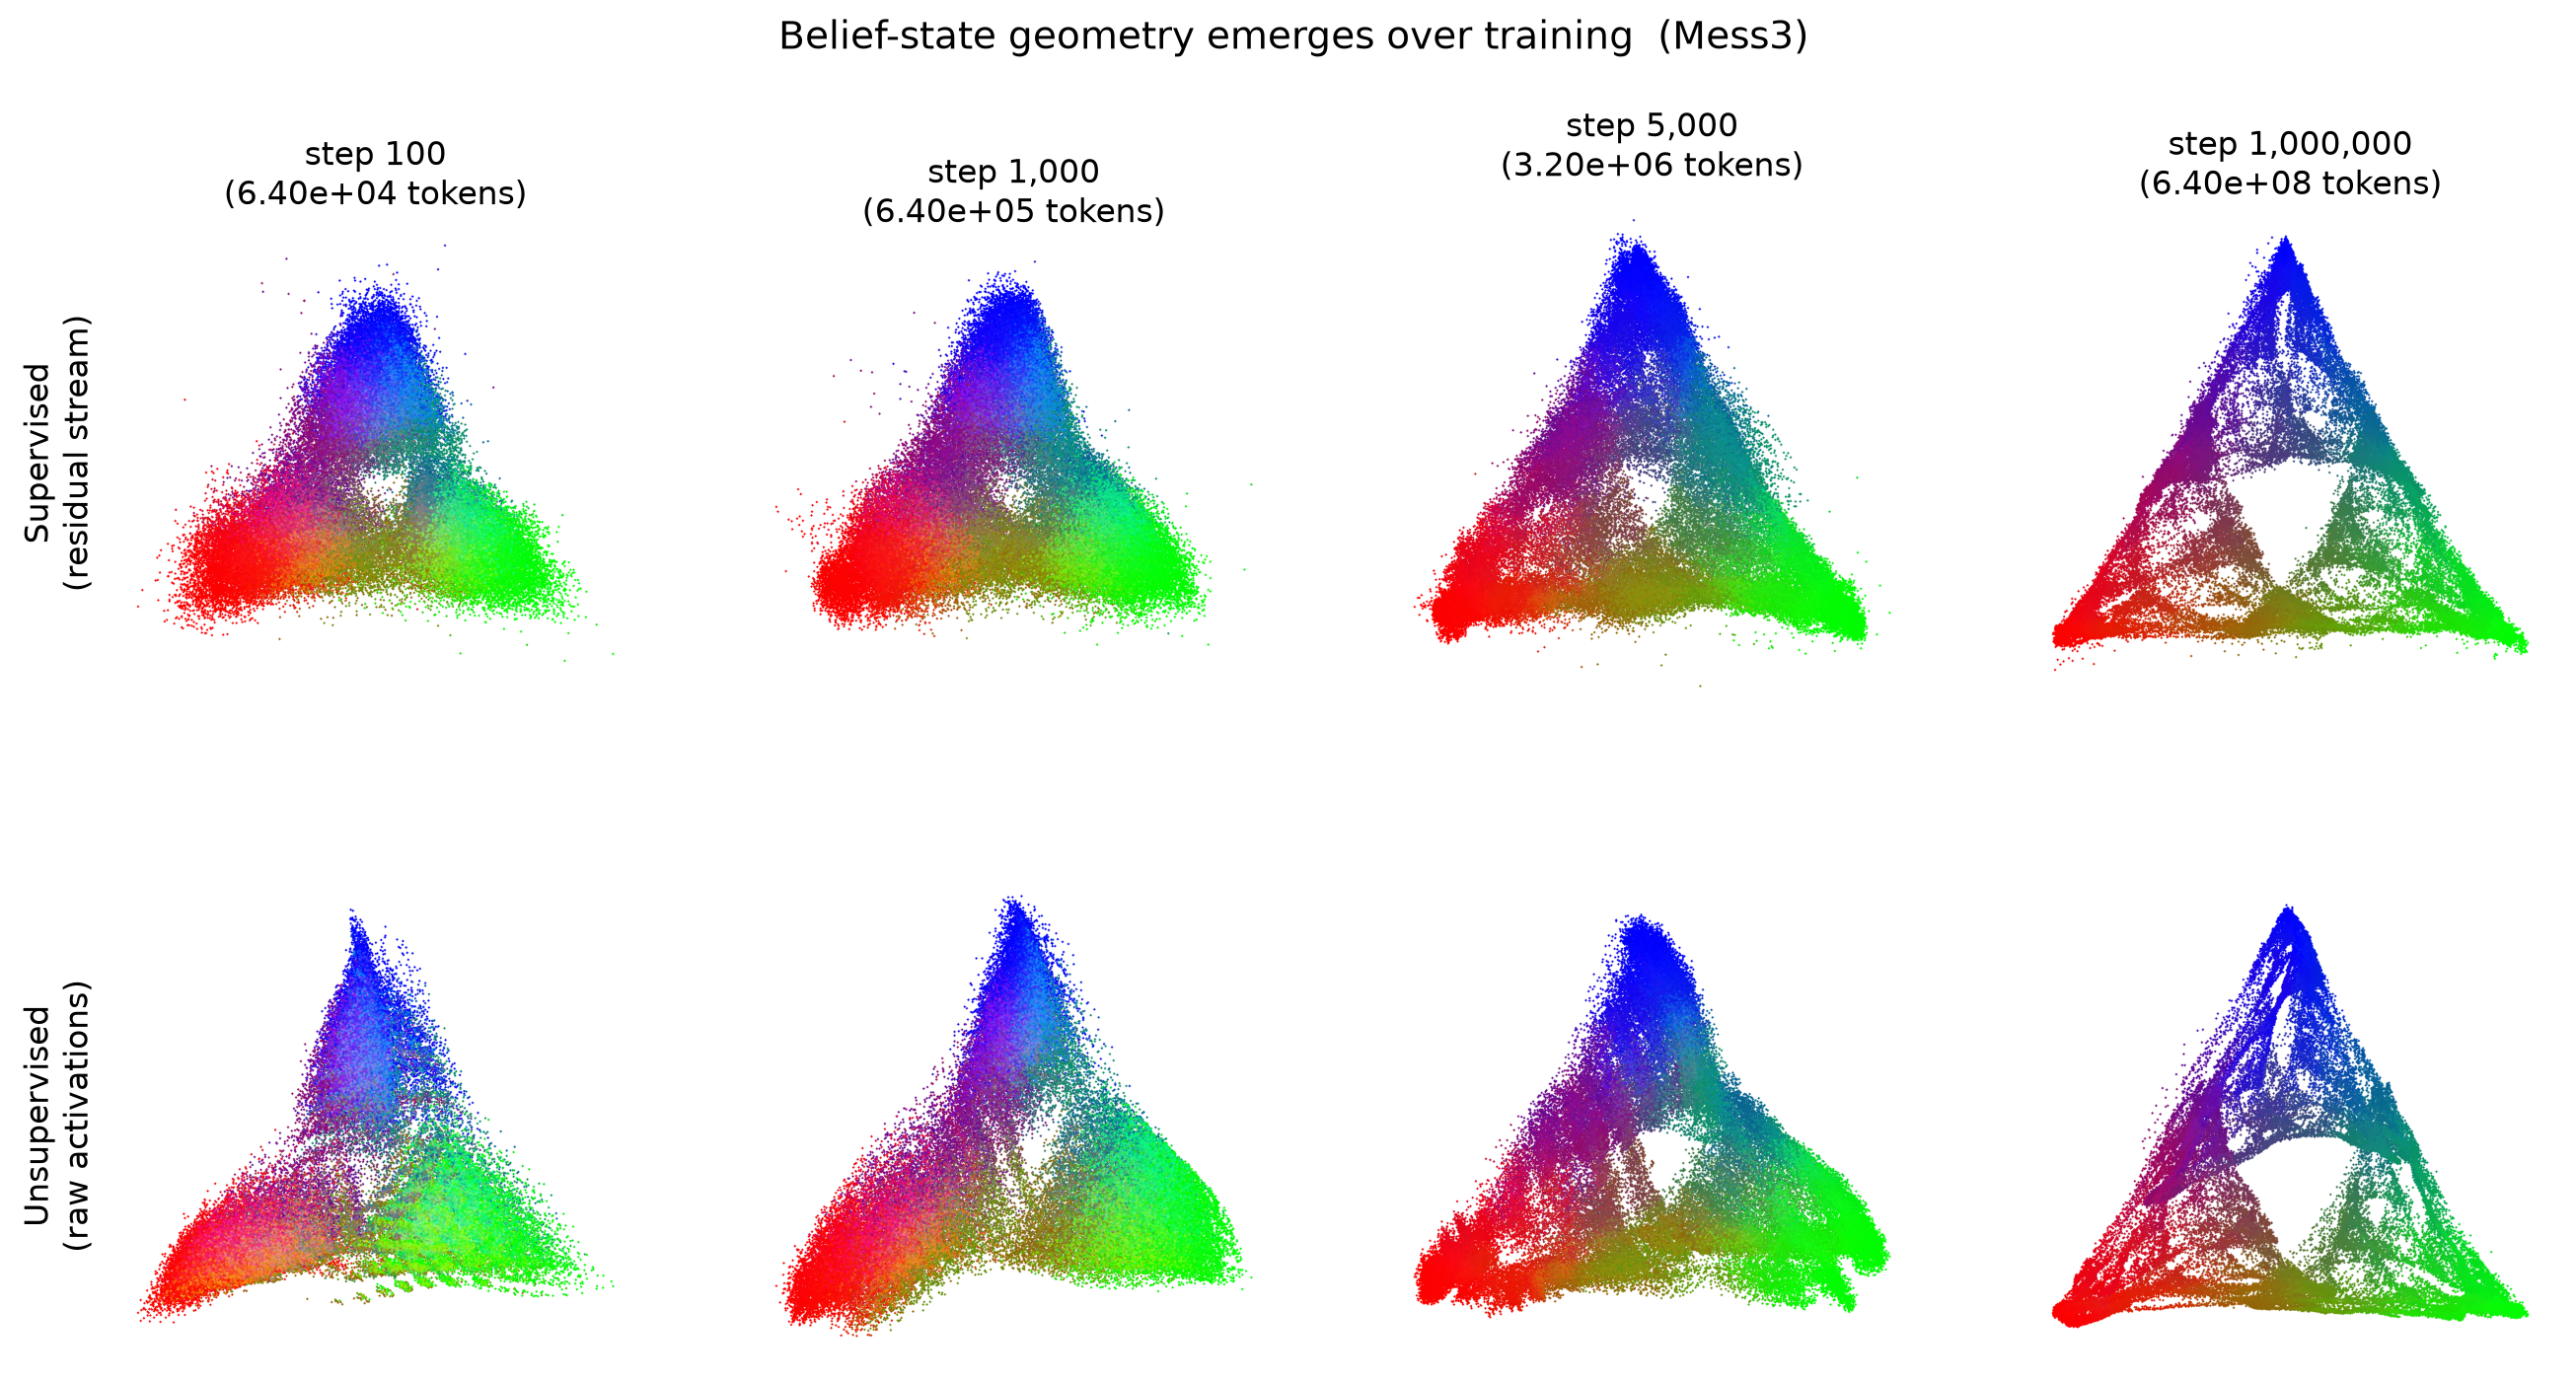
\includegraphics[width=0.8\textwidth]{fig2_training_progression_mess3.png}
\caption{\textbf{Mess3 emergence over training.}
Top: supervised decode at steps $100, 1000, 5000, 10^6$.
Bottom: spectral-OOM subspace activations (affine-aligned for display).
Both show identical emergence trajectory.}
\label{fig:mess3prog}
\end{figure}

\begin{figure}[!ht]
\centering
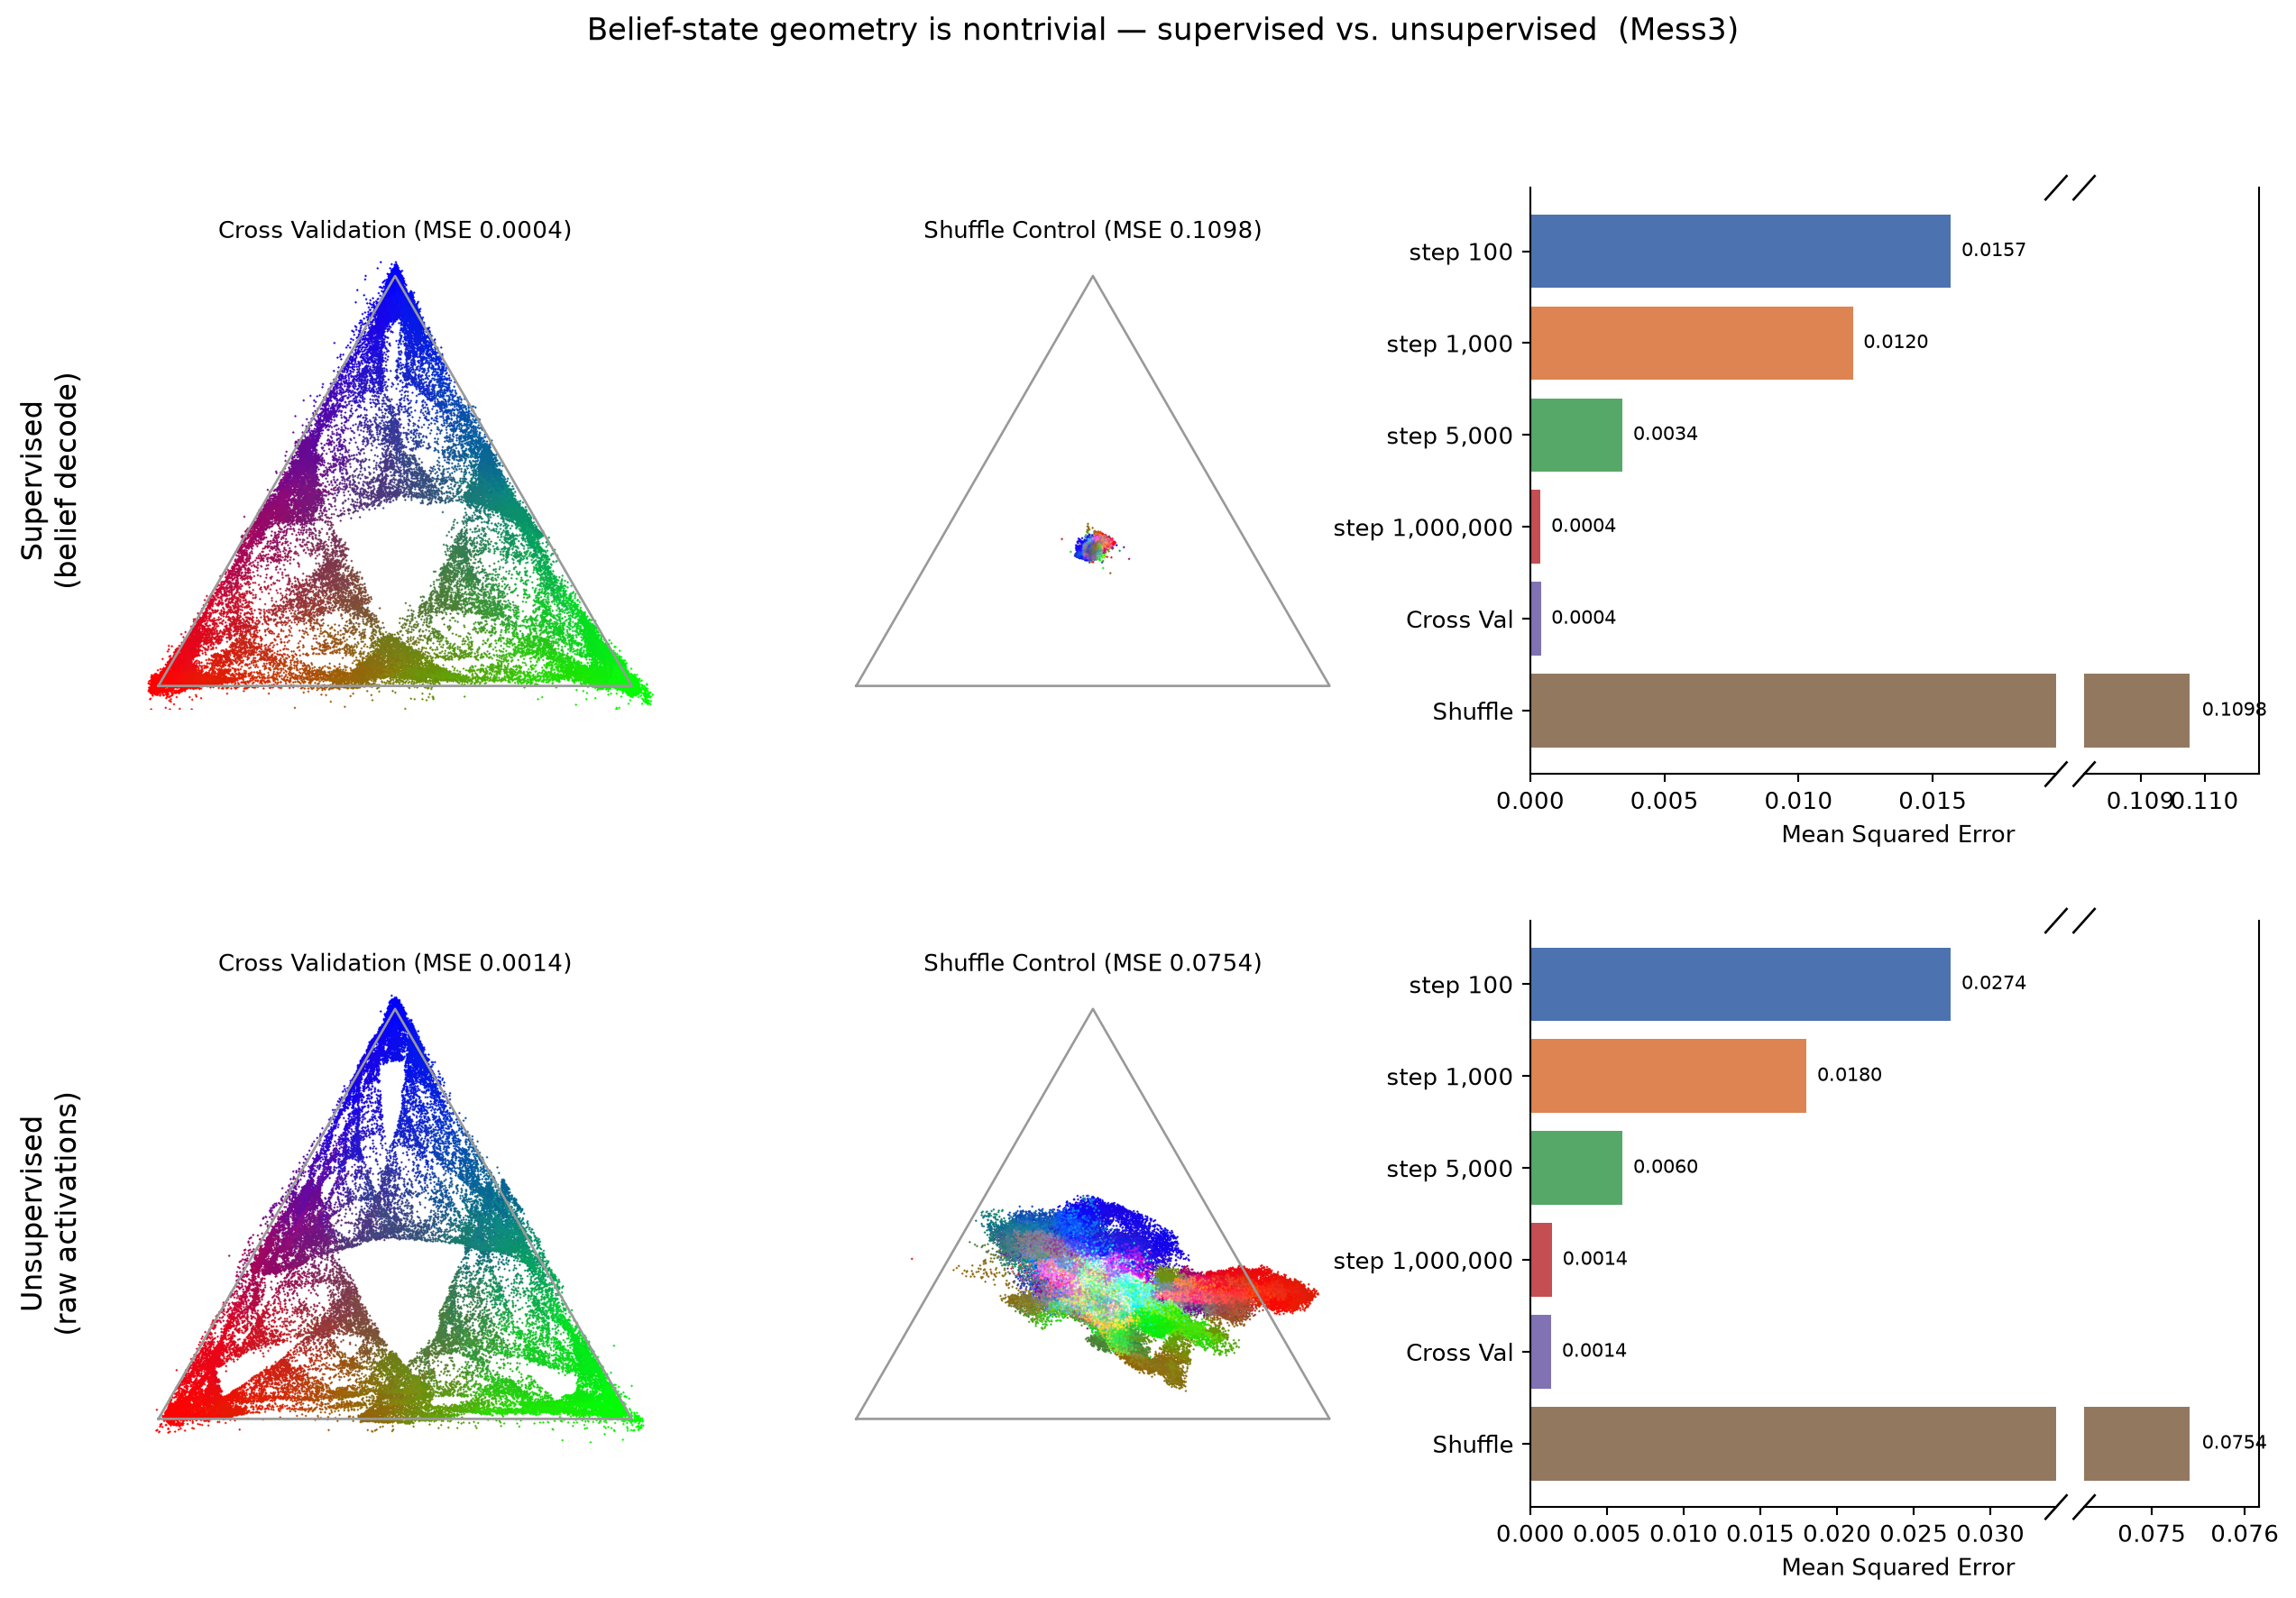
\includegraphics[width=0.8\textwidth]{fig3_unsupervised_controls_mess3.png}
\caption{\textbf{Mess3 controls: cross-validation and shuffle.}
Top: supervised.
Bottom: unsupervised.
Both recover the fractal on held-out prefixes (CV) and collapse dramatically under shuffle control.}
\label{fig:mess3ctrl}
\end{figure}

\subsection{RRXOR}
\label{sec:rrxor}

For RRXOR the gap to supervised recovery is substantial. The unsupervised subspace
recovers the diamond geometry but more diffusely (Figure~\ref{fig:rrxorcomp}). We report
two complementary scores: per-position $R^2$ (full point cloud) and state-level $R^2$ (36 belief state centers-of-mass). The unsupervised subspace gives
per-position $R^2=0.65$ (supervised $0.91$) and state-level $R^2=0.82$ (supervised $1.00$).
The $d=5$ dimension was fixed \textit{a priori} from the known RRXOR state count, since the
singular spectrum showed no clean elbow for this process.

\begin{figure}[!ht]
\centering
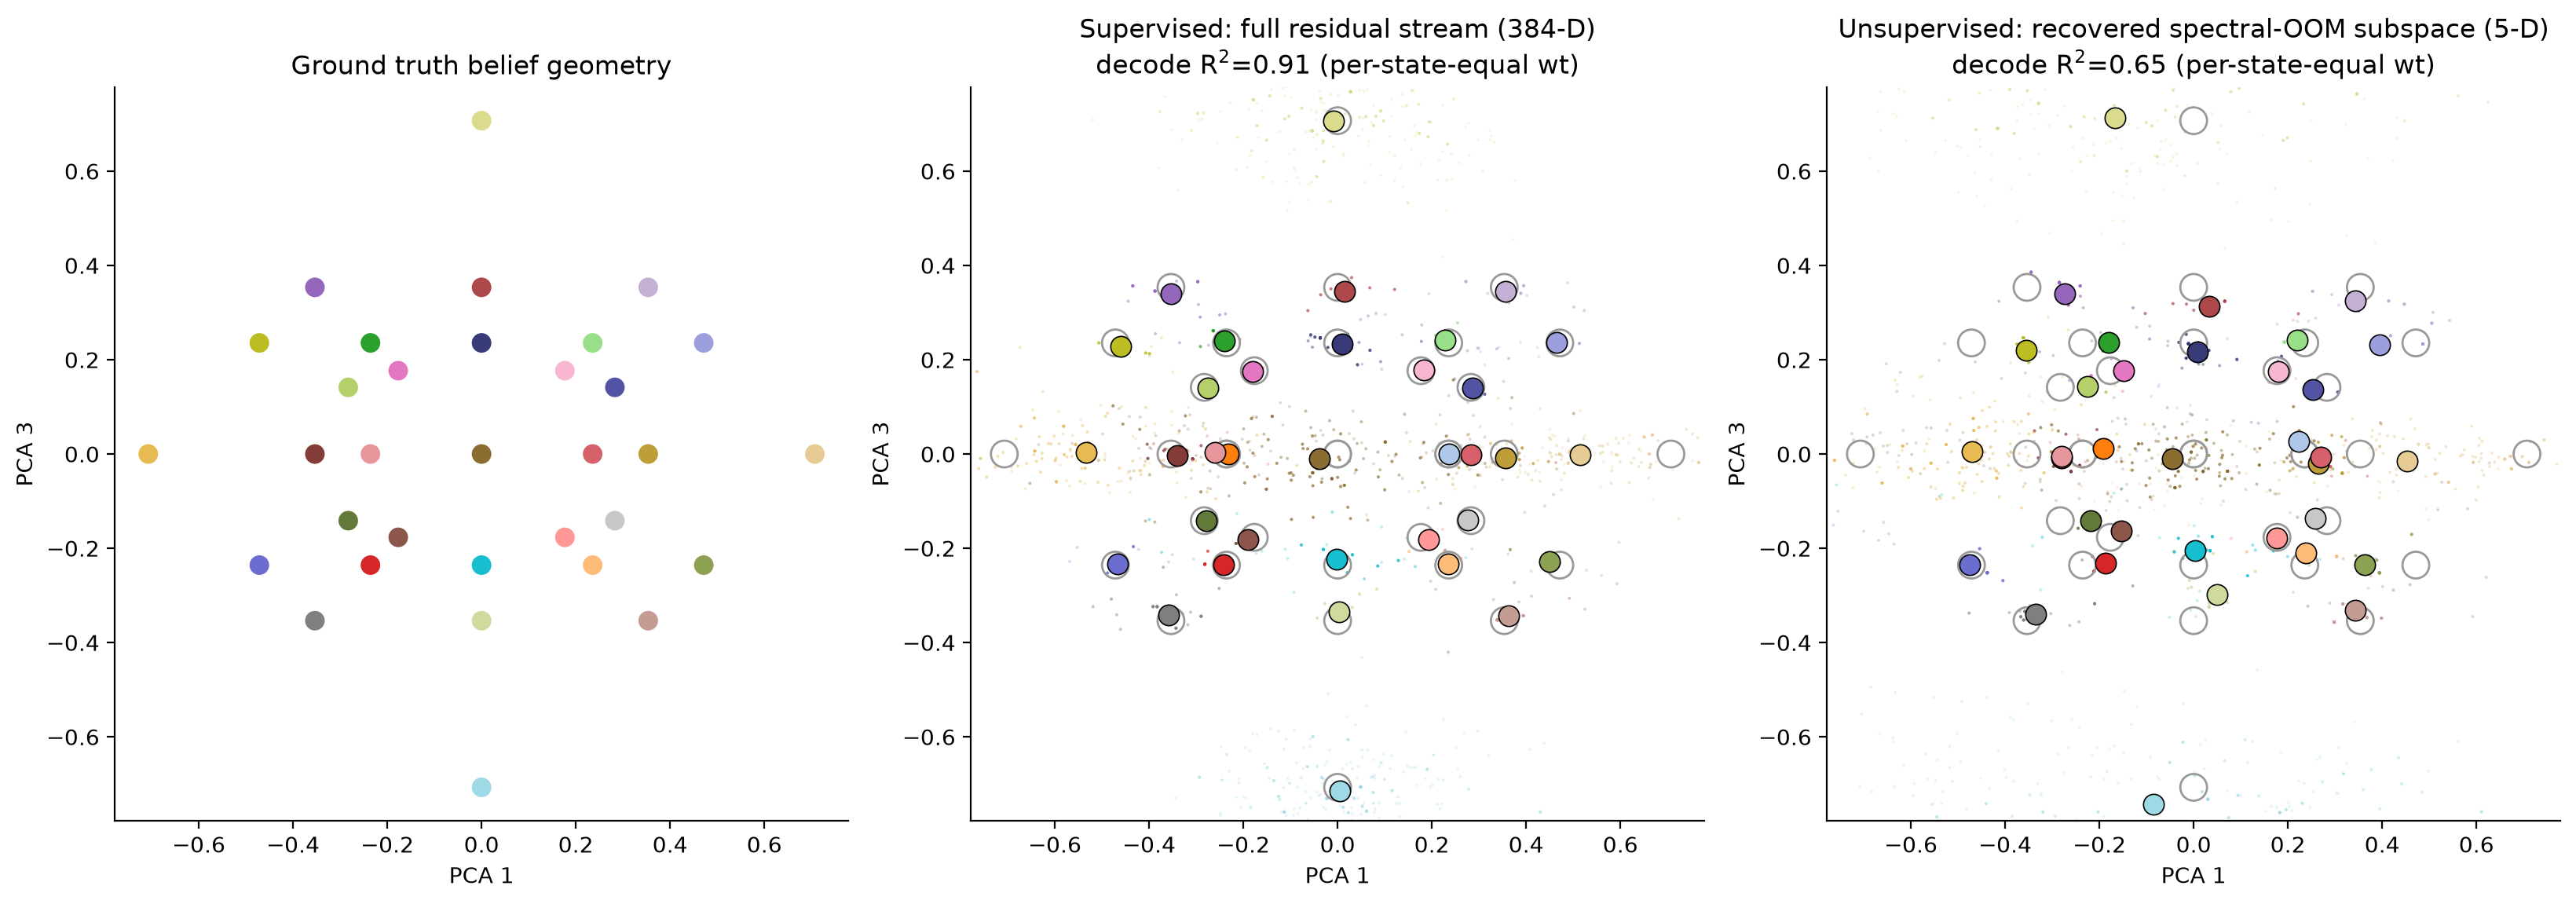
\includegraphics[width=0.9\textwidth]{fig4_rrxor_principled.png}
\caption{\textbf{RRXOR: ground truth, supervised, and unsupervised.}
Left: ground-truth $36$ belief states (PC1/PC3 plane, display only).
Centre: supervised decode (per-position $R^2=0.91$).
Right: recovered subspace (per-position $R^2=0.65$, state-level $R^2=0.82$).
The gap reflects weak observability.}
\label{fig:rrxorcomp}
\end{figure}
\bigskip
\noindent This gap is structural, not an artefact of estimator quality. The root cause is rank deficiency 
in the observability matrix: RRXOR's belief directions produce only faint singular values in 
the predictive observables (the multi-step version of the $0.33$ next-token limitation), making 
them difficult to recover unsupervised. We tested observability at horizons $L=3$ through $L=15$ with 
$P(w)$-weighting on the full length-10 enumeration. The state-level geometry $R^2$ at 
$d=5$ shows that longer horizons do not improve recovery, best performance is at $L=3$ ($R^2=0.815$). 
This confirms that observability is maximized at the shortest tested horizon.
\\\\
The layerwise analysis and distance preservation are recovered in the supervised case (Figure~\ref{fig:rrxordiag}).
Belief is spread across all layers (no single layer encodes it well), and is preserved in
distances better than next-token. Notably, the unsupervised representation reverses this (Figure~\ref{fig:rrxordiagU}).
Next-token distances ($R^2 \approx 0.68$) are preserved better than belief ($R^2 \approx 0.50$). A possible 
explanation for this might be that the spectral-OOM subspace is too biased towards the next-token observable $C$.
Since RRXOR's belief geometry is not strongly correlated with next-token structure, this method may not be 
well-poised to recover the true belief geometry.

\begin{figure}[!ht]
\centering
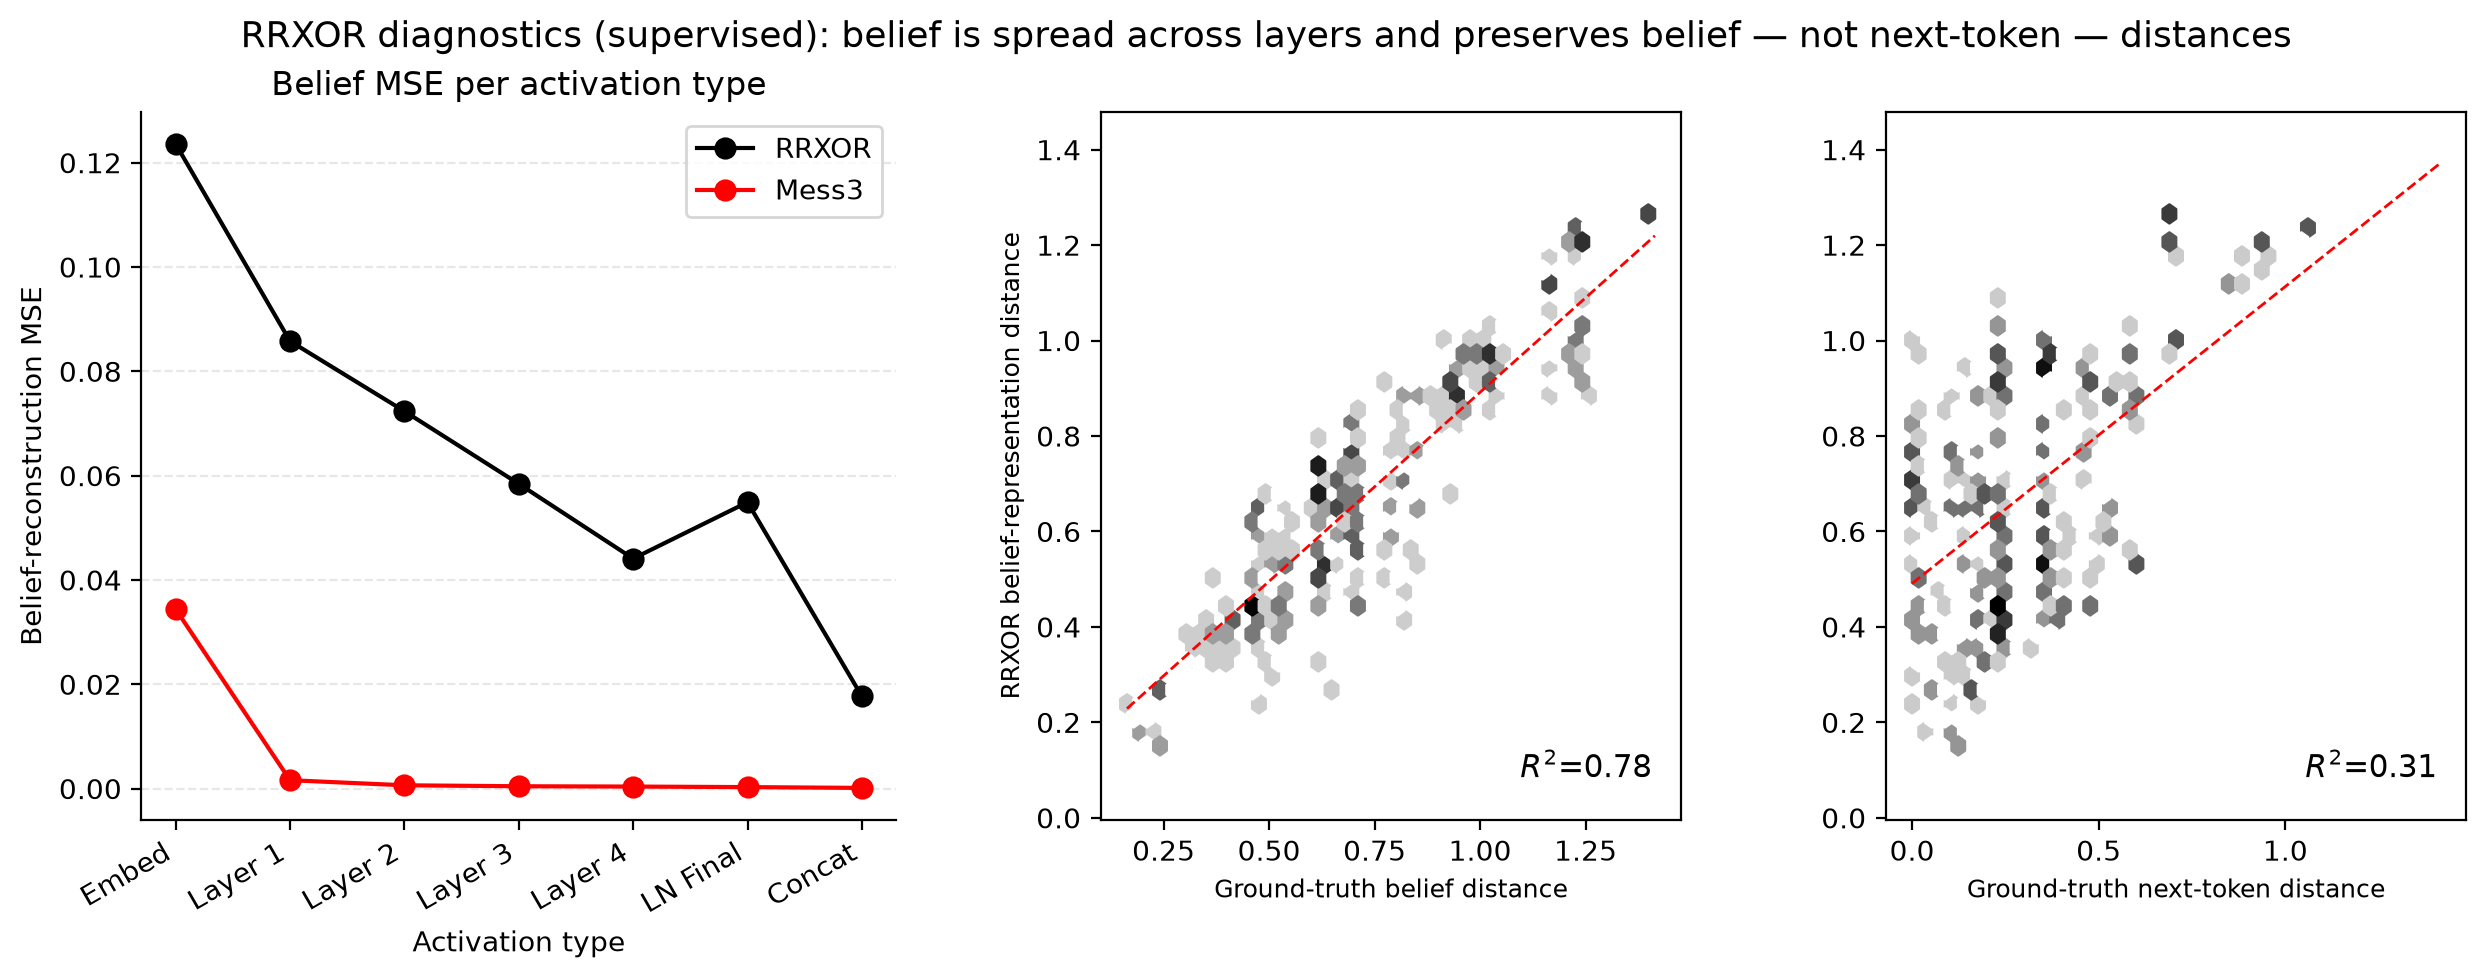
\includegraphics[width=0.9\textwidth]{fig5_rrxor_diagnostics_supervised.png}
\caption{\textbf{RRXOR diagnostics: supervised.}
Left: per-activation belief-reconstruction MSE.
Centre/right: belief and next-token distance preservation via hexbin.}
\label{fig:rrxordiag}
\end{figure}

\begin{figure}[!ht]
\centering
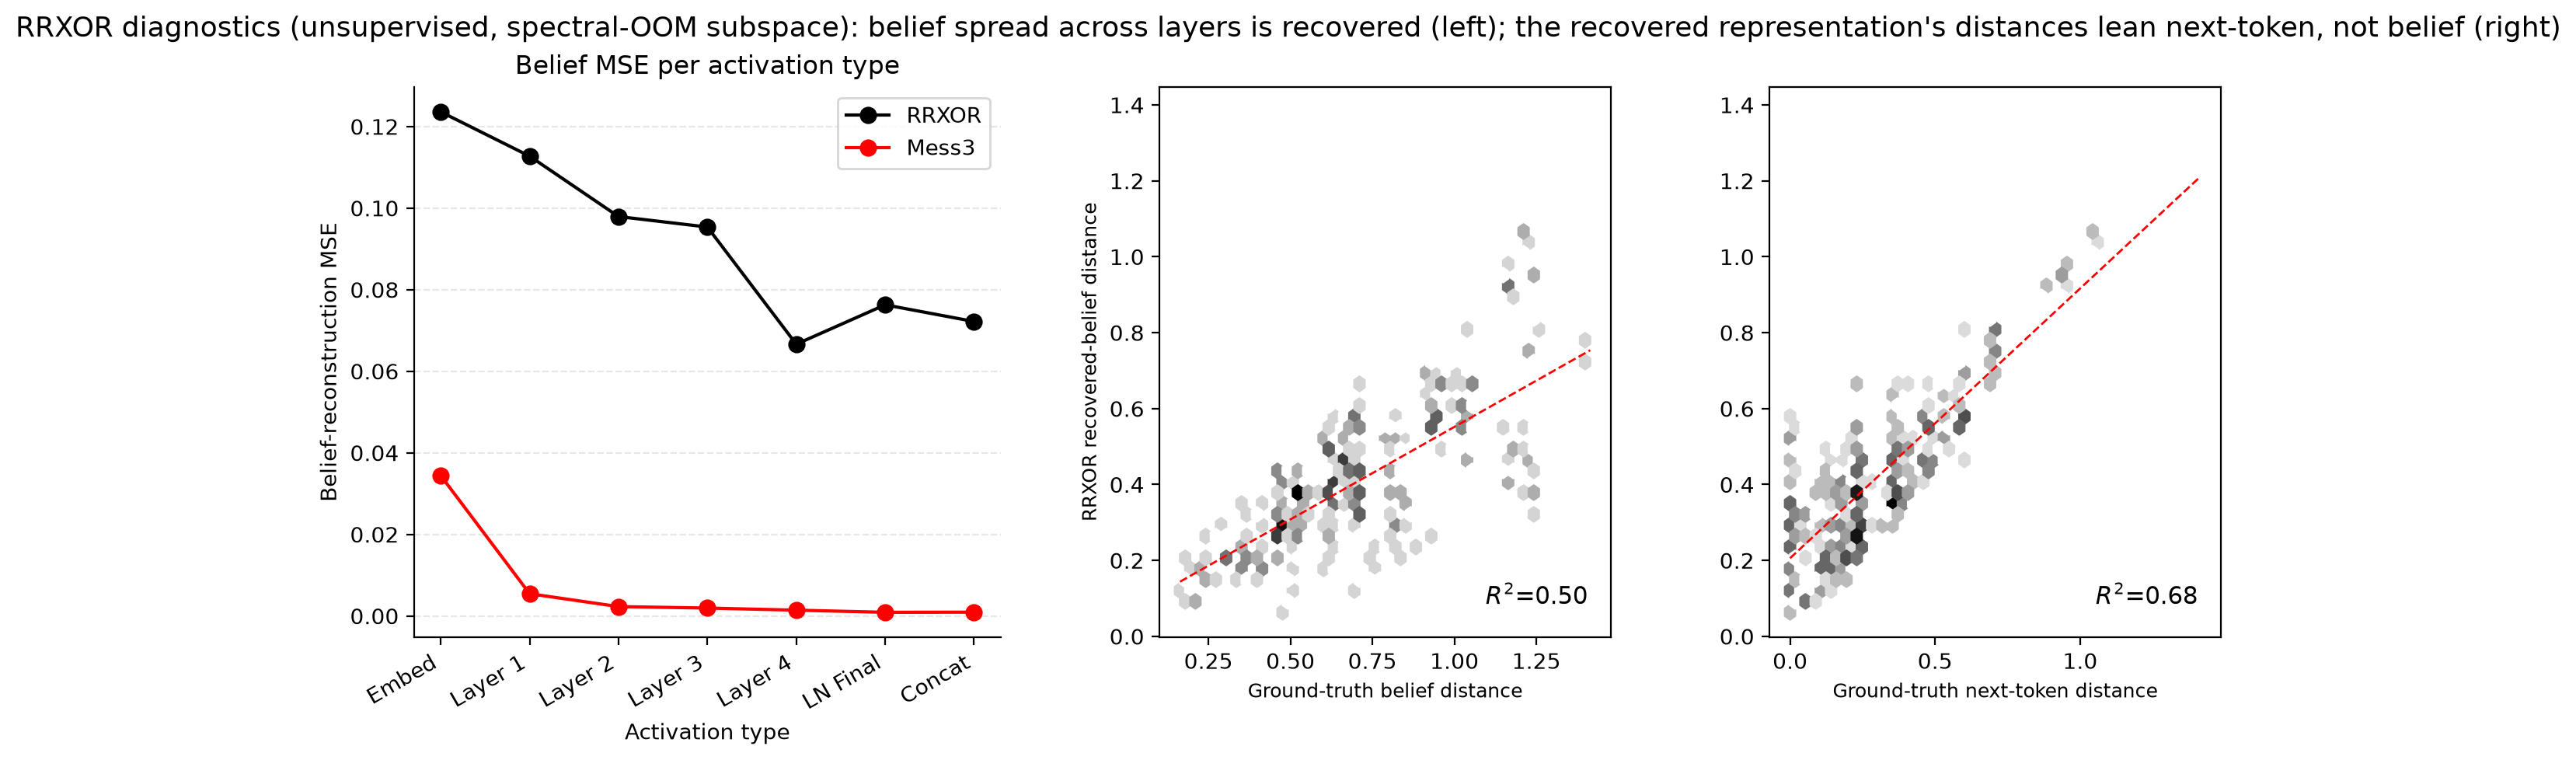
\includegraphics[width=0.9\textwidth]{fig6_rrxor_diagnostics_unsupervised.png}
\caption{\textbf{RRXOR diagnostics: unsupervised.}
Same metrics as Figure~\ref{fig:rrxordiag}, but from the recovered spectral-OOM subspace.
Belief spread is recovered, but next-token distances dominate.}
\label{fig:rrxordiagU}
\end{figure}

\section{Conclusion}

The belief-state geometry can be recovered unsupervised from activations and softmax alone,
nearly perfectly for Mess3 ($R^2 \approx 0.998$), but only partially for RRXOR (state-level $R^2 \approx 0.82$).
The spectral-OOM anchors to next-token predictions (the softmax observable), but RRXOR's belief states exhibit
significant next-token degeneracy because many geometrically distinct states share similar next-token distributions
($R^2 = 0.31$ from the original paper). It is unclear whether this can be fully addressed, as there are no obvious
alternative observables satisfying the required properties (linearity in belief, empirical accessibility). A longer
context window would reduce finite-sample error but not the underlying degeneracy. Success on Mess3 demonstrates the
method's viability where belief geometry aligns with observable structure, and a richly-sampled quantum or post-quantum
process is a natural next step. Even if the method never scales to large models, it remains useful across
the many small models whose belief geometry we can now study to learn what such geometry reveals about what 
a model has learned.

\appendix
\section{Observable Operator Models (OOMs): Spectral-OOM Estimator Details}

\subsection{The spectral-OOM estimator on transformer activations}

From Section ~\ref{sec:estimator}, the network encodes belief affinely: $a(w) = b(w)\Psi + c$.
Working in $P(w)$-centered coordinates (the offset $c$ is absorbed by the
regression intercept), the projective update~(\ref{eq:update}) is non-linear in $a$, but its
normaliser is precisely the softmax $P(x|w) = b(w)T^x\mathbf{1}$. Multiplying both sides by the
normaliser gives $b(wx)\,P(x|w) = b(w)T^x$; right-multiplying by $\Psi$
linearises the update:
\begin{equation}
a(w)\,A_x \approx P(x|w)\,a(wx), \qquad A_x=\Psi^{+}T^x\Psi .
\end{equation}

\paragraph{Building the observability matrix.}
Let $C$ be the ridge regression of activations onto the softmax (the one-step observable),
and $\{G_x\}$ the estimated transition operators (ridge regressions of activations onto
$P(x|w)\cdot$child-activations, i.e.\ the empirical version of $A_x$). All regressions are
$P(w)$-weighted to bias the estimator toward high-probability prefixes. Because each $G_x$
is linear in belief and composition preserves linearity, every block below is linear in
$b(w)$. Stacking multi-step observables to horizon $3$ gives the observability matrix
\begin{equation}
\mathcal{O}=\big[\,C \;\big|\; (G_x C)_{x} \;\big|\; (G_x G_y C)_{x,y}
\;\big|\; (G_x G_y G_z C)_{x,y,z}\,\big],
\end{equation}
indexed over all words up to length $3$. This is the (word-indexed) control-theoretic
observability matrix of the estimated OOM: with a single-symbol alphabet it reduces to the
classical Kalman form $[\,C \mid CA \mid CA^2 \mid \dots\,]$, and the token-indexed family
$\{G_x\}$ is the natural OOM/PSR generalisation. An SVD $\mathcal{O}=U\Sigma V^\top$ yields
the orthonormal basis $B=U_{:,1:d}$, with the numerical rank $d$ giving the model order.

\paragraph{What is and isn't unsupervised.}
Subspace choice, operator fit, and one-step $R^2$ are fully target-free (activations +
softmax only). Order selection is target-free where the spectrum has a clean elbow
(Mess3, $d=3$); for the weakly observable RRXOR there is no elbow, and $d=5$ is set a
priori from the known state count (Section~2.3). The final placement onto the simplex and
numerical comparisons use ground-truth beliefs, but only for display and scoring, not for
fitting.

\section{Operator Rollouts}

A stronger test of the subspace is the generative \emph{operator rollout}. The
activation-space operators $A_x$ of Eq.~\eqref{eq:linearise} were used only to build the
observability matrix and locate the subspace; they are not iterated. The rollout instead
asks whether a self-contained dynamical system fitted \emph{inside} the recovered subspace
can regenerate the entire geometry from the root alone.
\\\\
Three steps produce it. (i)~\emph{Operator-consistency refit}: the recovered basis $B$ is
good for decoding but is not exactly closed under the rescaled-transition relation, so
operators fitted in it drift when iterated; we refine $B$ by alternating least squares
(ALS) into an operator-consistent basis $B_{\mathrm{op}}$, alternating between fitting
operators in the current basis and rotating the basis toward one those operators map into
itself.

\subsection{Results}

\textbf{Mess3:} the rollout reproduces the full fractal at $R^2 \approx 1.00$ from both supervised
and unsupervised subspaces (Figures \ref{fig:mess3suproll} and \ref{fig:mess3unsuproll}).
Mess3's true operators are diagonalisable strict contractions. The fractal is their attractor, so 
errors contract away and the rollout self-corrects

\begin{figure}[!ht]
\centering
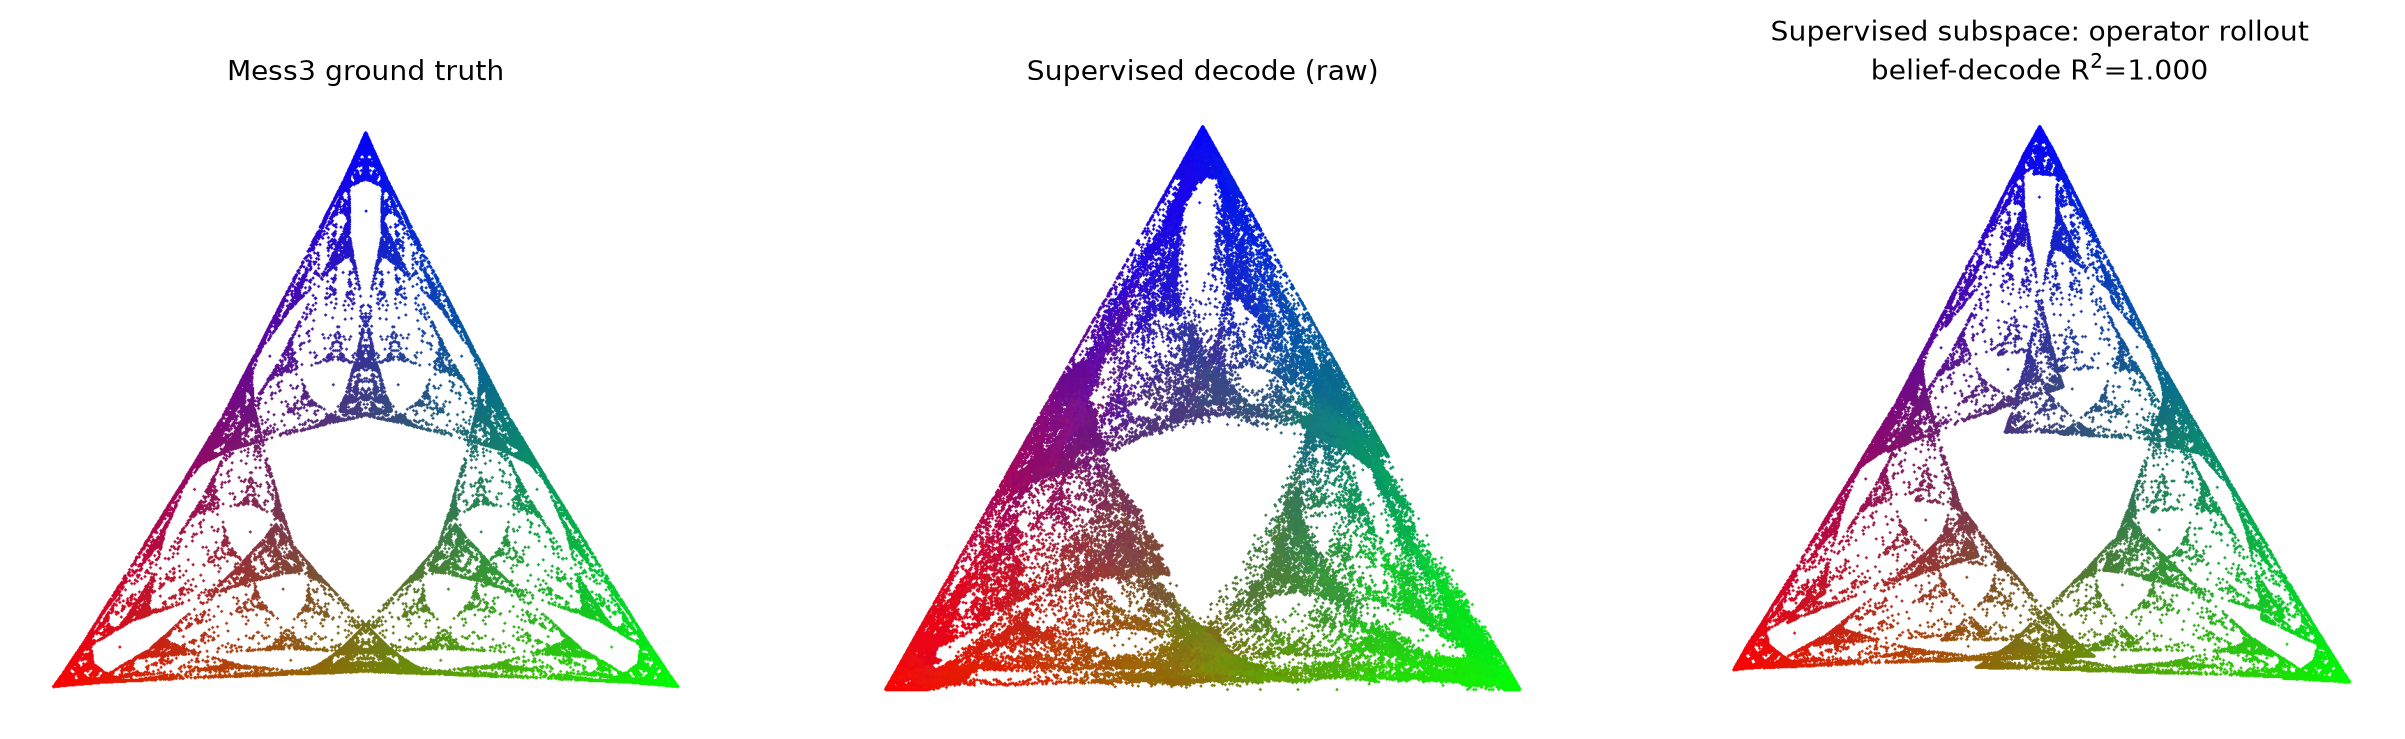
\includegraphics[width=0.9\textwidth]{fig7_mess3_supervised_rollout.png}
\caption{\textbf{Mess3 supervised subspace.}
Ground truth $|$ supervised decode $|$ operator rollout ($R^2=1.00$).}
\label{fig:mess3suproll}
\end{figure}

\begin{figure}[!ht]
\centering
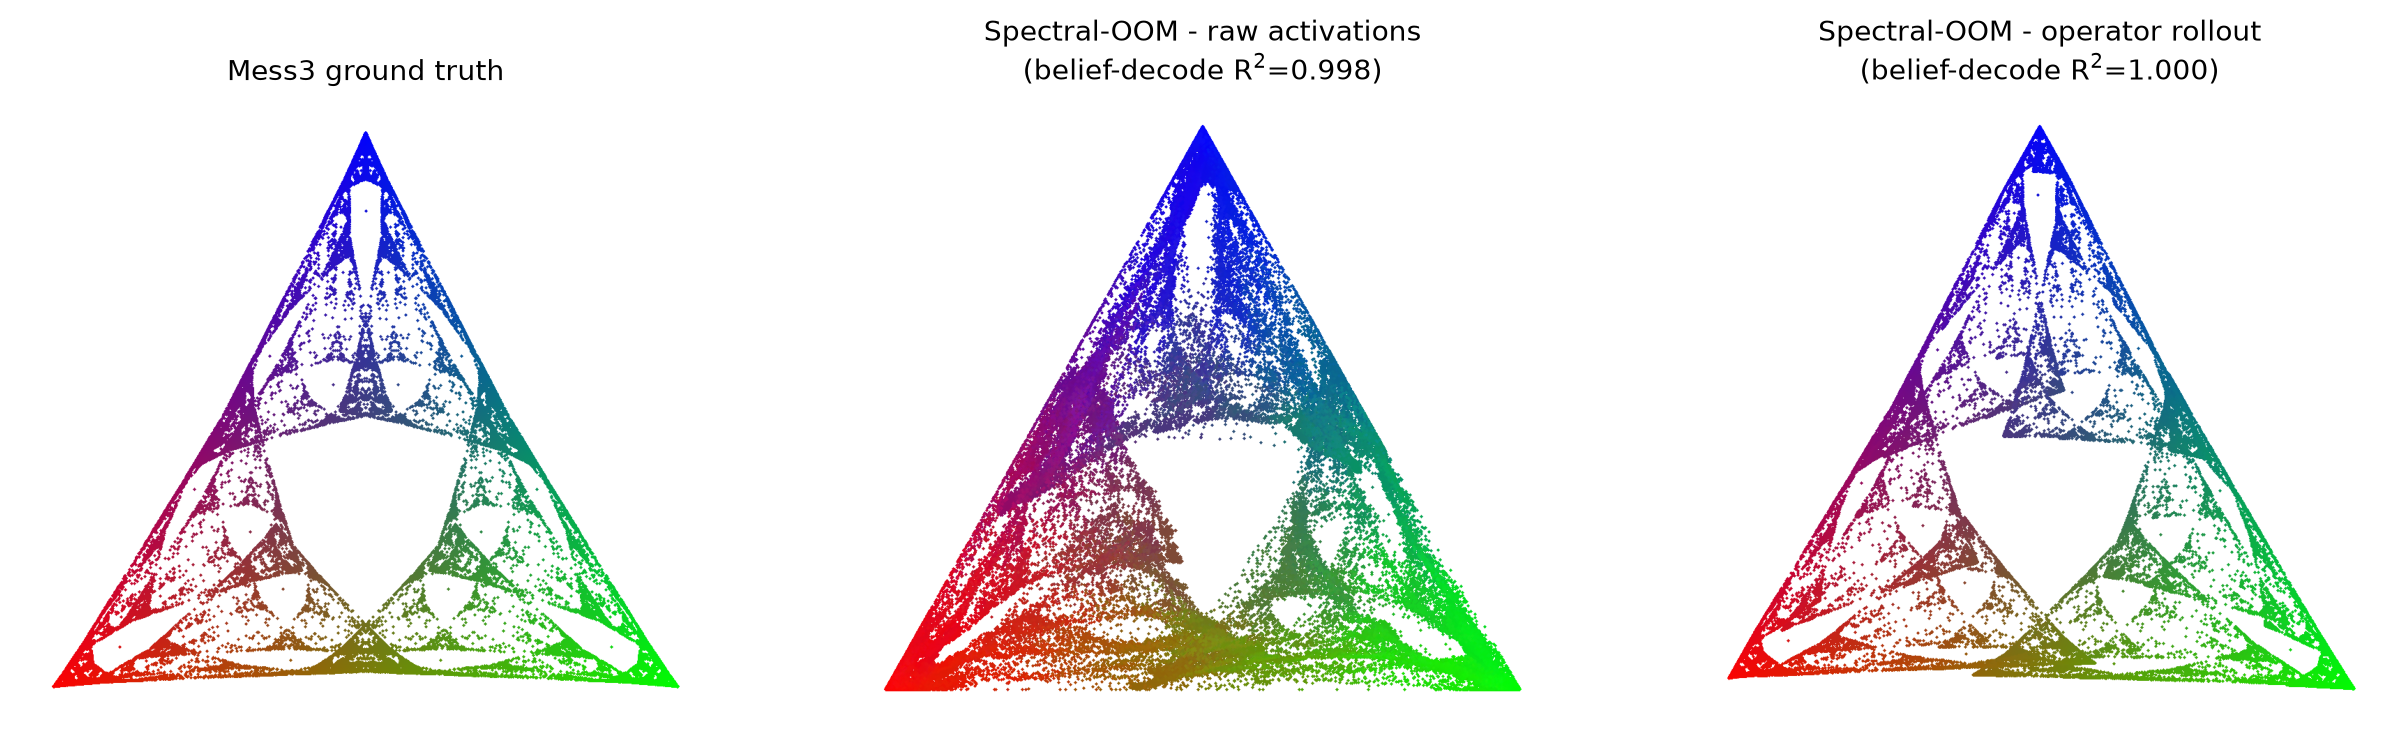
\includegraphics[width=0.9\textwidth]{fig8_mess3_unified.png}
\caption{\textbf{Mess3 spectral-OOM subspace.}
Ground truth $|$ recovered subspace (raw) $|$ operator rollout via $\widehat{A}_x$ ($R^2=1.00$).}
\label{fig:mess3unsuproll}
\end{figure}
\bigskip
\noindent\textbf{RRXOR:} the rollout collapses, failing to reach the outer apexes from both supervised
and unsupervised subspaces (Figures \ref{fig:rrxorsuproll} and \ref{fig:rrxorunsuproll}).
This is intrinsic to RRXOR's operator algebra: both of the transition operators
$T_x$ are non-diagonalisable; the input-$1$ operator is nilpotent
($T_1^{\,5}=0$), the input-$0$ operator is defective with a repeated
eigenvalue, so the belief states are transient points the dynamics passes through, not a
contractive attractor it settles onto and self-corrects toward. The rollout operators $\widehat{A}_x$, 
fitted to approximate this dynamics, reproduce the same behaviour. With no
attractor to contract onto, iteration accumulates error and the extreme apex
states are never reached.

\begin{figure}[!ht]
\centering
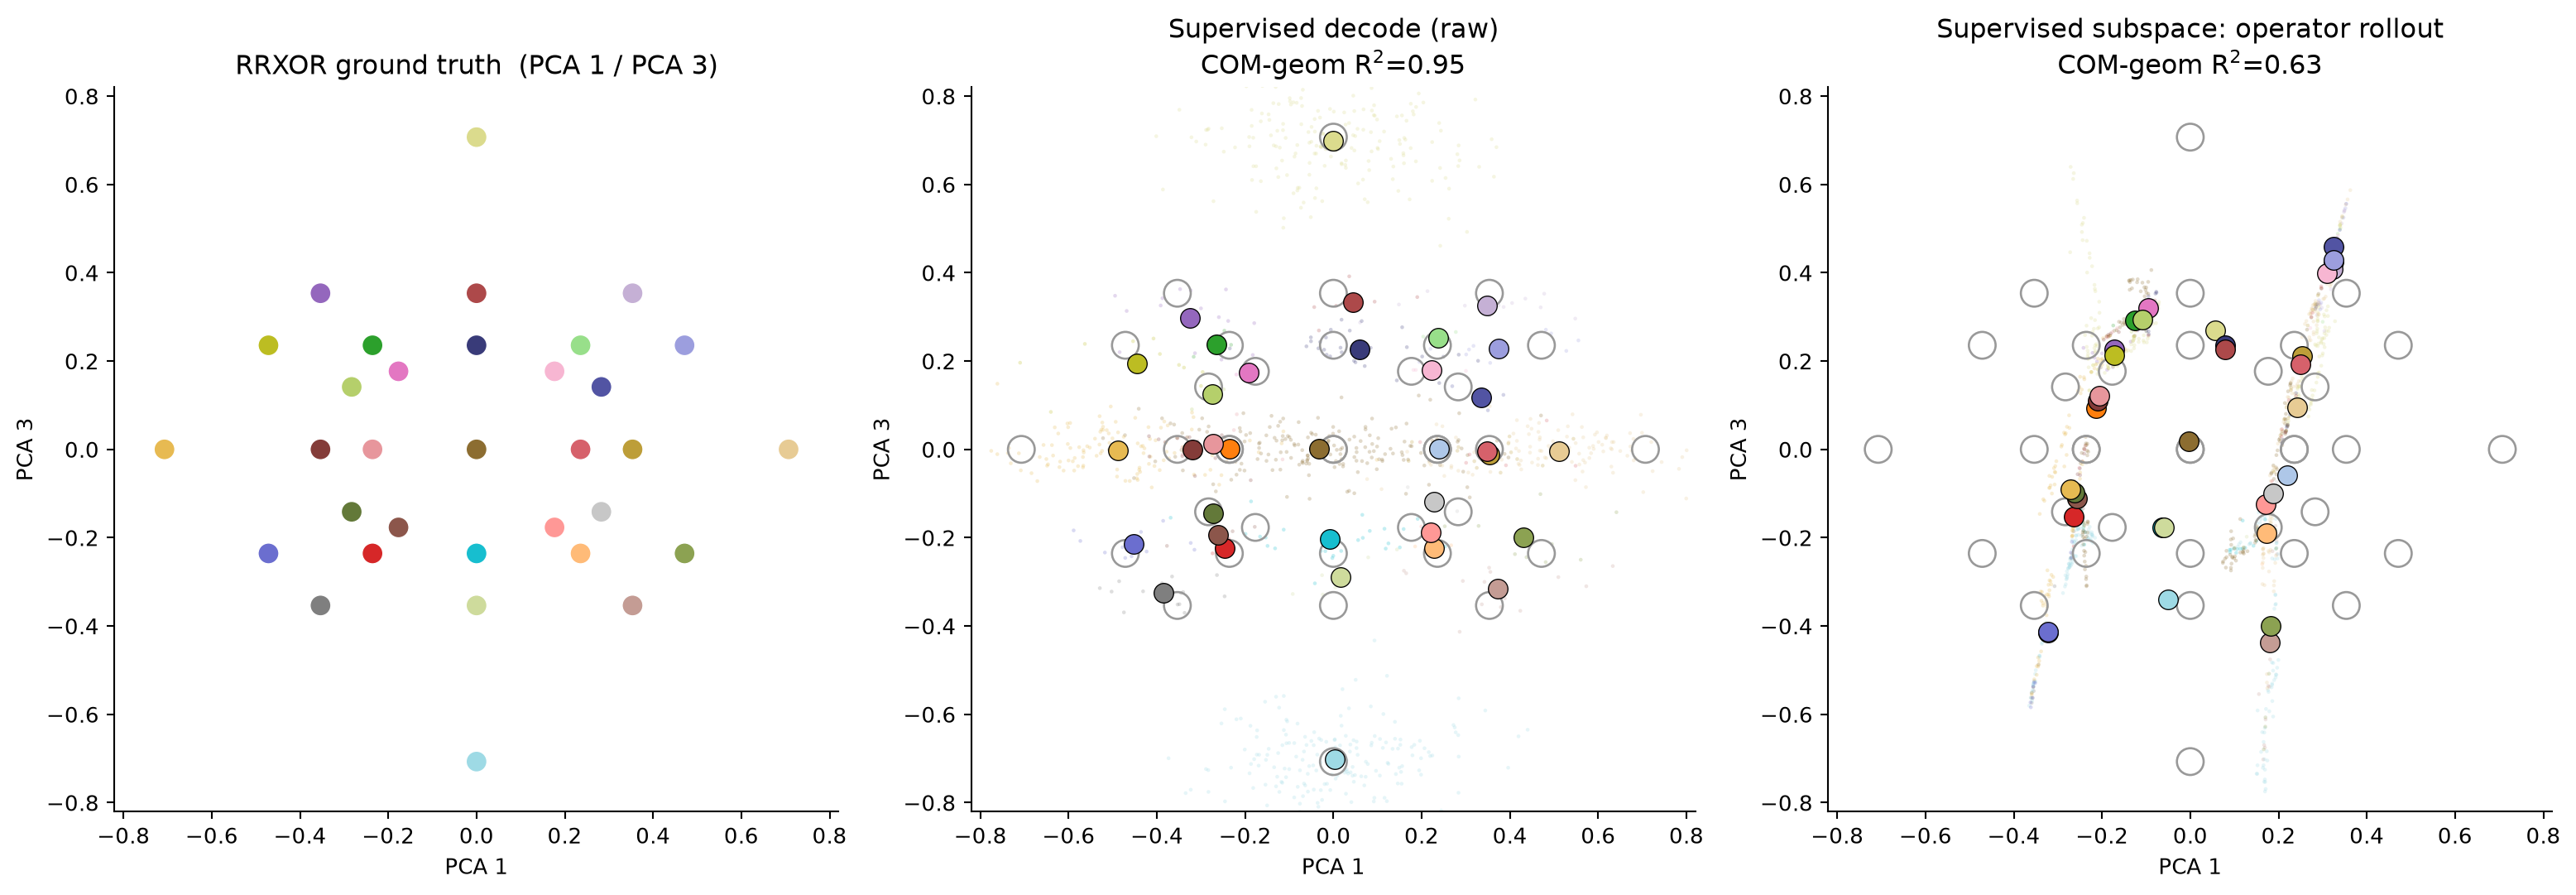
\includegraphics[width=0.9\textwidth]{fig9_rrxor_supervised_rollout.png}
\caption{\textbf{RRXOR supervised subspace.}
Ground truth $|$ supervised decode (COM-geom $0.95$) $|$ operator rollout (COM-geom $0.63$;
extreme states not reached).}
\label{fig:rrxorsuproll}
\end{figure}

\begin{figure}[!ht]
\centering
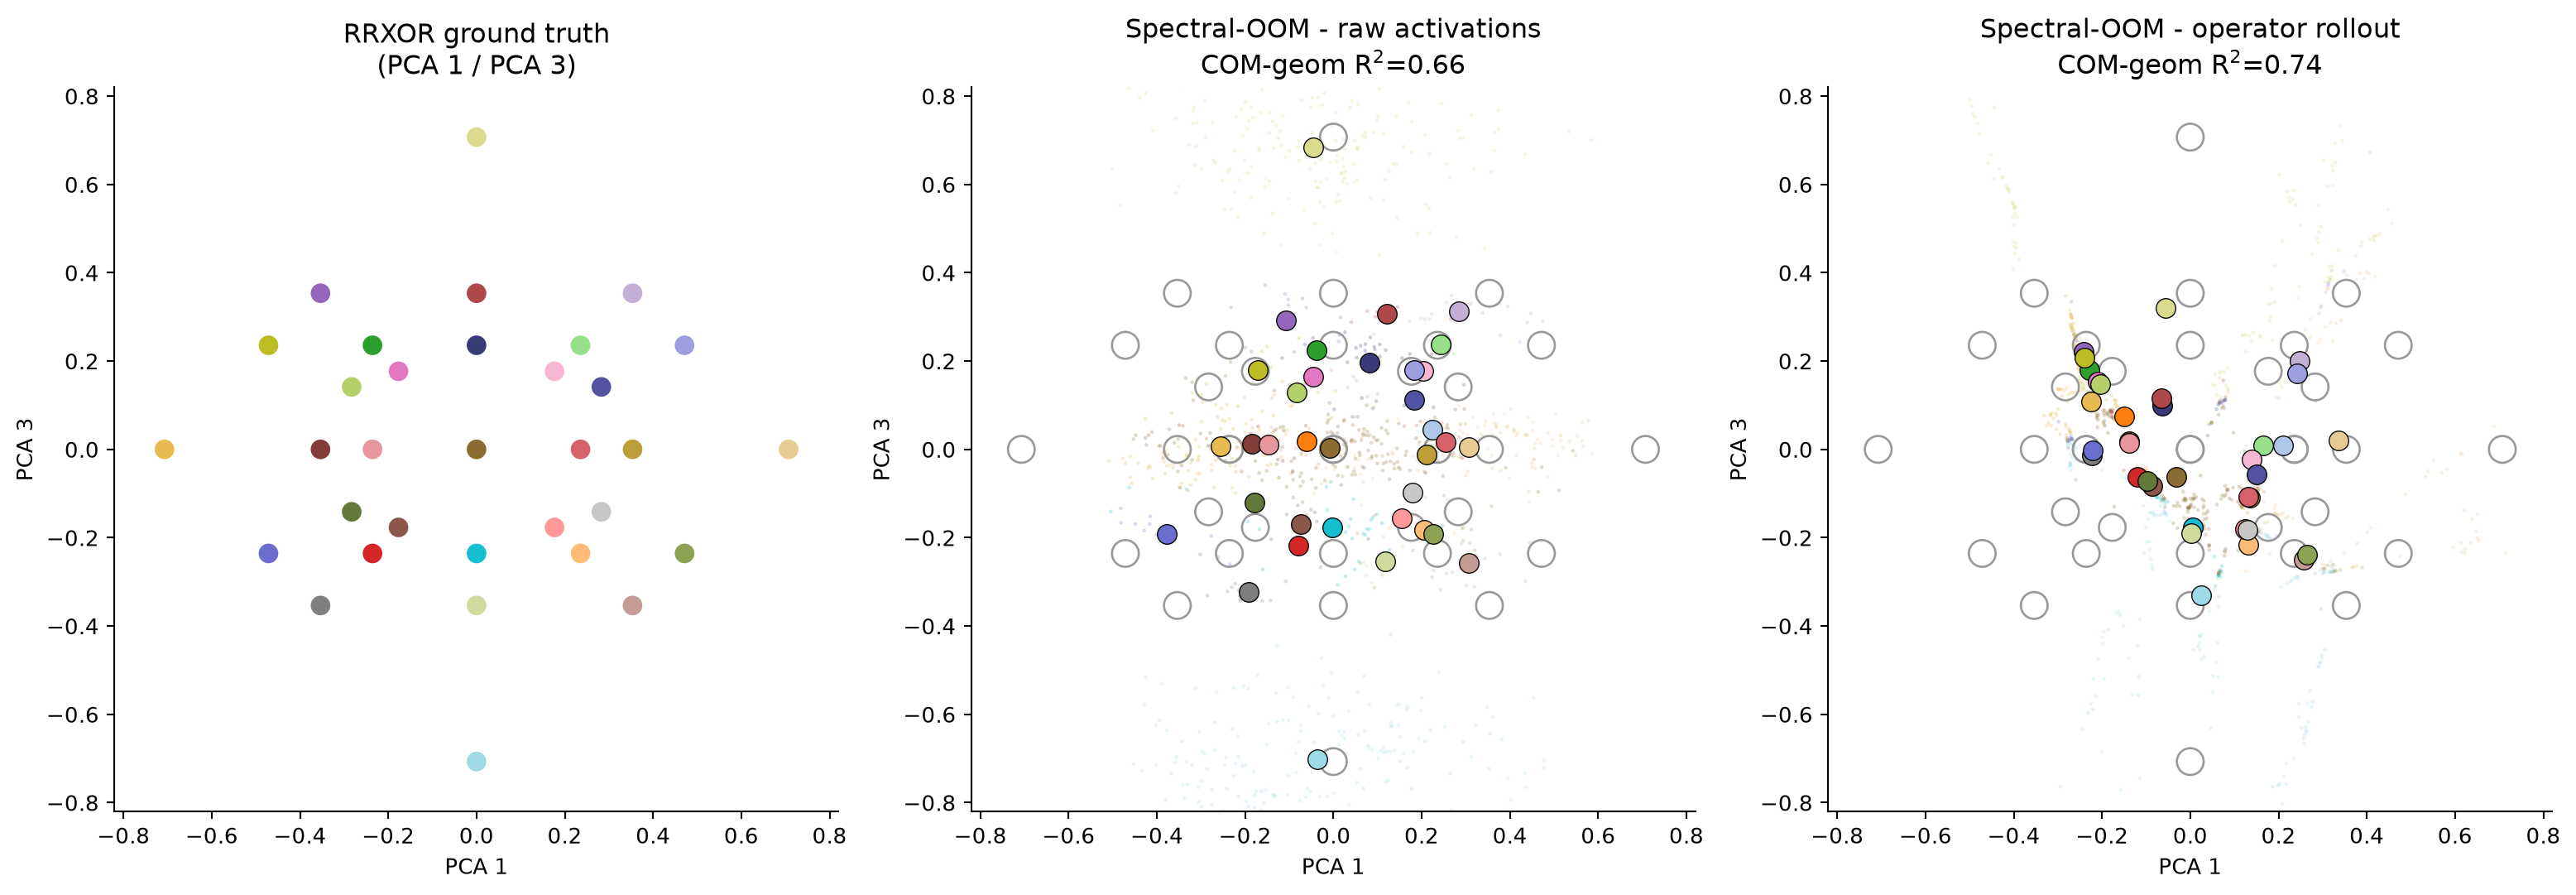
\includegraphics[width=0.9\textwidth]{fig10_rrxor_unified.png}
\caption{\textbf{RRXOR spectral-OOM subspace.}
Ground truth $|$ recovered subspace (raw, state-level $R^2=0.66$) $|$ operator rollout via
$\widehat{A}_x$ (state-level $R^2=0.74$; extreme states central).}
\label{fig:rrxorunsuproll}
\end{figure}

\newpage
\begin{thebibliography}{9}
\small
\bibitem{shai2024} A.~S. Shai, S.~E. Marzen, L.~Teixeira, A.~G. Oldenziel, P.~M. Riechers.
\emph{Transformers represent belief state geometry in their residual stream.}
NeurIPS 2024; arXiv:2405.15943.
\bibitem{riechers2025} P.~M. Riechers, T.~J. Elliott, A.~S. Shai.
\emph{Neural networks leverage nominally quantum and post-quantum representations.}
arXiv preprint arXiv:2507.07432, 2025.
\bibitem{baum1970} L.~E. Baum, T.~Petrie, G.~Soules, N.~Weiss.
\emph{A maximization technique occurring in the statistical analysis of probabilistic functions of Markov chains.}
Annals of Mathematical Statistics 41(1):164--171, 1970.
\bibitem{jaeger2000} H.~Jaeger.
\emph{Observable operator models for discrete stochastic time series.}
Neural Computation 12(6):1371--1398, 2000.
\bibitem{thon2015} M.~Thon, H.~Jaeger.
\emph{Links between multiplicity automata, observable operator models and predictive state
representations --- a unified learning framework.}
JMLR 16:103--147, 2015.
\bibitem{hsu2012} D.~Hsu, S.~M. Kakade, T.~Zhang.
\emph{A spectral algorithm for learning hidden Markov models.}
J.\ Computer and System Sciences 78(5):1460--1480, 2012.
\bibitem{littman2001} M.~L. Littman, R.~S. Sutton, S.~Singh.
\emph{Predictive representations of state.}
NeurIPS 2001.
\bibitem{crutchfield1989} J.~P. Crutchfield, K.~Young.
\emph{Inferring statistical complexity.}
Physical Review Letters 63(2):105--108, 1989.
\bibitem{shalizi2001} C.~R. Shalizi, J.~P. Crutchfield.
\emph{Computational mechanics: Pattern and prediction, structure and simplicity.}
J.\ Statistical Physics 104:817--879, 2001.
\end{thebibliography}

\end{document}
